%        File: prac2.tex
%     Created: Sun Mar 03 05:00  2019 S
% Last Change: Sun Mar 03 05:00  2019 S
%
\documentclass[a4paper, 12pt]{article}
\usepackage[]{amsmath}
\usepackage{amssymb}
\usepackage{float}
\usepackage[]{graphicx}
\usepackage{subfig}
\usepackage{caption}


\title{Control Systems 4A Practical 2 Report}
\author{Ruan de Bruyn, 216054484 \and Quintin Kruger, 216008466}

\begin{document}

\pagenumbering{gobble}
\begin{titlepage}
  \maketitle
\end{titlepage}

\pagenumbering{roman}
\tableofcontents
\newpage
\pagenumbering{arabic}

\section{Question 1}
\subsection{Input-Output form}
From the schematic representation of a DC motor, we can use KVL in order to
find the input-output relationships of all the components in the circuit
expressed as voltages. This leaves us with

\begin{equation}
  \begin{array}{rcl}
    v & = & V_R + V_L + e \\
    & = & Ri + L\dot i + K \dot\theta
  \end{array}
  \label{eq:KVL}
\end{equation}

\noindent Note that \eqref{eq:KVL} is a better representation for us to solve
the input-output equations; the current through the DC Motor is also the
same current through the other components. From theory, we can relate the
back-emf of the motor to its rotational speed $\dot\theta$ with the constant
$K$, as well as expressing the current in the DC Motor with the following
equation:

\begin{equation}
  J\ddot\theta + b\dot\theta = Ki \Rightarrow i = \tfrac{J}{K} \ddot\theta + \tfrac{b}{K}\dot\theta
  \label{eq:dc_current}
\end{equation}

From \eqref{eq:KVL} and \eqref{eq:dc_current}, and letting $\dot\theta = \omega$, we get

\begin{equation}
  Kv = LJ\ddot\omega + (Lb + RJ)\dot\omega + (Rb + K^2)\omega
  \label{eq:final_voltage}
\end{equation}

From \eqref{eq:final_voltage}, if we want to express the equation in terms of
in input reference rotational speed $\omega_r$, then we can evaluate equation
\eqref{eq:final_voltage} by assuming that $\omega_r$ is steady state, and thus
that its derivatives are zero. We then come to an expression for voltage in
terms of $\omega_r$ as:

\begin{equation}
  \begin{array}{rcl}
    Kv & = & (Rb + K^2)\omega_r \\
    v & = & \frac{(Rb + K^2)\omega_r}{K}
  \end{array}
  \label{eq:ref_omega}
\end{equation}

Finally, substituting equation \eqref{eq:ref_omega} into
\eqref{eq:final_voltage}, we get our final input-output equation as

\begin{equation}
  (Rb + K^2)\omega_r = LJ\ddot\omega + (Lb + RJ)\dot\omega + (Rb + K^2)\omega
  \label{eq:final_ref_omega}
\end{equation}

\subsection{State-variable Matrix form}
In order to represent our system in state-variable matrix form, we choose to
model it with parameters $\omega$ and $i$. For the first equation of the
state-variable representation, we require $\dot\omega$ and $\dot i$. We get the
former by rearranging \eqref{eq:dc_current}, taking $\dot\theta = \omega$,
which yields

\begin{equation}
  \dot\omega = \frac{K}{J} i - \frac{b}{J} \omega
  \label{eq:ss_omega_dot}
\end{equation}

Similarly, we rearrange \eqref{eq:KVL}, and substitute \eqref{eq:ref_omega} to
get

\begin{equation}
  \begin{array}{rcl}
    Ri + L\dot i + K\omega & = & v \\
    Ri + L\dot i + K\omega & = & \frac{(Rb + K^2)}{K}\omega_r \\
    \dot i & = & \frac{(Rb + K^2)}{KL}\omega_r - \frac{R}{L} i - \frac{K}{L}\omega \\
  \end{array}
  \label{eq:ss_i_dot}
\end{equation}

Now we can get the state-variable equations as

\begin{equation}
  \left[
  \begin{array}{c}
    \dot \omega \\
    \dot i
  \end{array}
  \right]
  =
  \left[
  \begin{array}{cc}
    -\frac{b}{J} & \frac{K}{J} \\
    -\frac{K}{L} & -\frac{R}{L}
  \end{array}
  \right]
  \left[
  \begin{array}{c}
    \omega \\
    i
  \end{array}
  \right]
  +
  \left[
  \begin{array}{c}
    0 \\
    \frac{Rb + K^2}{LK}
  \end{array}
  \right]
  \left[
  \begin{array}{c}
    \omega_r
  \end{array}
  \right]
  \label{eq:ss_eq1}
\end{equation}

\begin{equation}
  y =
  \left[
  \begin{array}{cc}
    1 & 0
  \end{array}
  \right]
  \left[
  \begin{array}{c}
    \omega \\
    i
  \end{array}
  \right]
  +
  \left[
  \begin{array}{c}
    0
  \end{array}
  \right]
  \left[
  \begin{array}{c}
    \omega_r
  \end{array}
  \right]
  \label{eq:ss_eq2}
\end{equation}

\subsection{Transfer Function form}

From equation \eqref{eq:final_ref_omega}, we can derive the transfer function
of the system in terms of reference angular velocity by taking the Laplace
Transform:

\begin{equation}
  \begin{array}{rcl}
    \mathcal{L}[(Rb + K^2)\omega_r] & = & \mathcal{L}[LJ\ddot\omega + (Lb + RJ)\dot\omega + (Rb + K^2)\omega] \\
    (Rb + K^2)\Omega_r & = & [LJs^2 + (Lb + RJ)s + (Rb + K^2)]\Omega \\
  \end{array}
  \label{eq:ts_initial}
\end{equation}

From equation \eqref{eq:ts_initial}, we can get the transfer function as

\begin{equation}
  T(s) = \frac{\Omega}{\Omega_r} = \frac{Rb + K^2}{LJs^2 + (Lb + RJ)s + Rb + K^2}
  \label{eq:ts_final}
\end{equation}

\subsection{Block Form}

Why would you even make us do this on an actual report?



\section{Question 2}
In order to have position control for a motor as well, we simply add an
additional state variable, $\theta$, and then go back to expressing all the
equations in the previous section in terms of $\theta$, instead of $\omega$. In
Question 1, we used the substitution $\omega = \dot\theta$ because there were
no terms of the equation that actually contained $\theta$ as is. So, for
brevity, we omit the derivation, as it is virtually the same as for Question 1,
and alter our existing state-variable equations to accommodate $\theta$, and
applying $\dot\theta = \omega$ to get

\begin{equation}
  \left[
  \begin{array}{c}
    \dot \theta \\
    \dot \omega \\
    \dot i
  \end{array}
  \right]
  =
  \left[
  \begin{array}{ccc}
    0 & 1 & 0 \\
    0 & -\frac{b}{J} & \frac{K}{J} \\
    0 & -\frac{K}{L} & -\frac{R}{L}
  \end{array}
  \right]
  \left[
  \begin{array}{c}
    \theta \\
    \omega \\
    i
  \end{array}
  \right]
  +
  \left[
  \begin{array}{c}
    0 \\
    0 \\
    \frac{Rb + K^2}{LK}
  \end{array}
  \right]
  \left[
  \begin{array}{c}
    \omega_r
  \end{array}
  \right]
  \label{eq:ss_position_eq1}
\end{equation}

\begin{equation}
  y =
  \left[
  \begin{array}{rcl}
	  y_1 \\
	  y_2
  \end{array}
  \right]
  =
  \left[
  \begin{array}{ccc}
    1 & 0 & 0 \\
    0 & 1 & 0
  \end{array}
  \right]
  \left[
  \begin{array}{c}
    \theta \\
    \omega \\
    i
  \end{array}
  \right]
  +
  \left[
  \begin{array}{c}
    0 \\
    0
  \end{array}
  \right]
  \left[
  \begin{array}{c}
    \omega_r
  \end{array}
  \right]
  \label{eq:ss_position_eq2}
\end{equation}

By using octave's \texttt{ss2tf} function and giving it as parameters matrices A through D which is the state space represenation of the DC motor using the code that follows, the step response is shown by Figure \ref{fig:question_2_output_response}\par

\noindent
\texttt{A = [0,1,0;0,(-b/J),(K/J); 0 -(K/L),-(R/L)];}\\
\texttt{B = [0;0;(R\*b + K\^2)/(L\*K)];}\\
\texttt{C = [1,0,0;0,1,0];}\\
\texttt{D = [0;0];}\\
\texttt{[num,den] = ss2tf(A,B,C,D);}\\
\texttt{H = tf(num,den);}\\
\texttt{step(H);}\\

\begin{figure}[H]
	\centering
	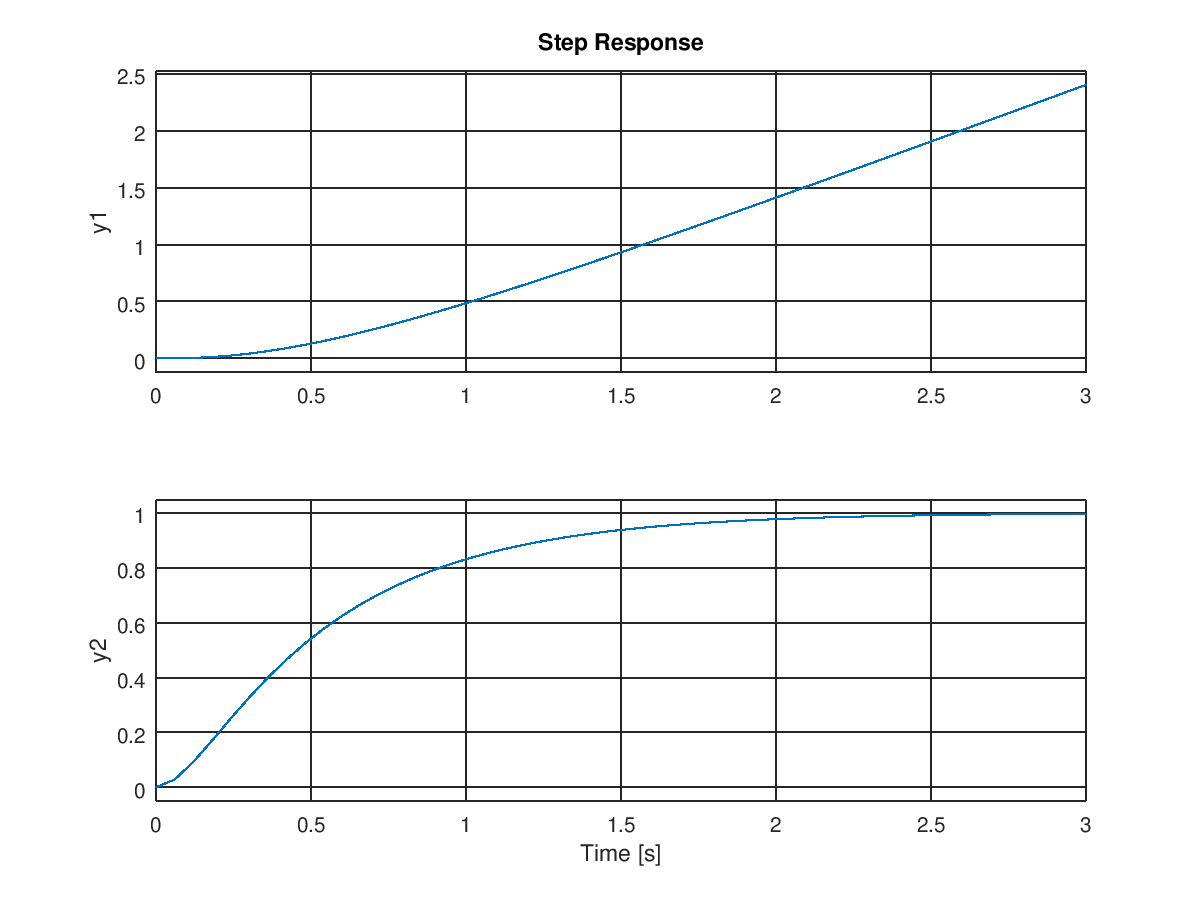
\includegraphics[width=\textwidth]{Images/question_2_output_response.png}
	\caption{Output response to a step input}
	\label{fig:question_2_output_response}
\end{figure}

Figure \ref{fig:question_2_output_response} shows the reponse of the sytem where $y_1$ is the angular displacement of the motor and $y_2$ is the angular speed of the motor. $y_1$ follows a linear relationship with time after transients of $y_2$ die out. This is expected seeing as though $y_2$ illustrates the rate of change of $y_1$, a constant rate of change (after roughly $2.5$ seconds) gives a linear relationship of the displacement. 

Before the transients die out, the displacement output $y_1$ shows to have a parabolic relationship with time. This is expected as the rate of change of disaplacement increases between the time $t=0$ seconds and $t=2.5$ seconds.    


\section{Question 3}

As given in the practical, the equation for current is slightly modified by
letting $\omega_r$ be evaluated as an error instead, due to the negative
feedback loop, thus replacing $\omega_r$ with $K_p[\omega_r(t) - \omega(t)]$.
The current equation then simply becomes

\begin{equation}
	\dot i = -\left[ \frac{K}{L} + \frac{K_P(Rb + K^2)}{LK} \right]\omega - \frac{R}{l}i + \frac{K_P(Rb + K^2)}{LK}\omega_r
	\label{eq:3_current}
\end{equation}

We can modify equation \eqref{eq:ss_position_eq1} to be

\begin{equation}
  \left[
  \begin{array}{c}
    \dot \theta \\
    \dot \omega \\
    \dot i
  \end{array}
  \right]
  =
  \left[
  \begin{array}{ccc}
    0 & 1 & 0 \\
    0 & -\frac{b}{J} & \frac{K}{J} \\
    0 & -\left[ \frac{K}{L} + \frac{K_P(Rb + K^2)}{LK} \right] & -\frac{R}{L}
  \end{array}
  \right]
  \left[
  \begin{array}{c}
    \theta \\
    \omega \\
    i
  \end{array}
  \right]
  +
  \left[
  \begin{array}{c}
    0 \\
    0 \\
    \frac{K_P(Rb + K^2)}{LK}
  \end{array}
  \right]
  \left[
  \begin{array}{c}
    \omega_r
  \end{array}
  \right]
  \label{eq:3_ss_position}
\end{equation}

The output system is exactly the same as in equation \eqref{eq:ss_position_eq2}.

By implementing this in Octave with the code that follows, the reponse changes to settle at a value of the proportional gain as shown by Figure \ref{fig:question_3_output_response_kp_1} and Figure \ref{fig:question_3_output_response_kp_01}\\
\noindent
\texttt{A = [0,1,0;0,(-b/J),(K/J); 0 -((K/L)+(Kp\*(R\*b+K\^2)/L\*K)),-(R/L)];}\\
\texttt{B = [0;0;Kp\*(R\*b + K\^2)/(L*K)];}\\
\texttt{C = [1,0,0;0,1,0];}\\
\texttt{D = [0;0];}\\
\texttt{[num,den] = ss2tf(A,B,C,D);}\\
\texttt{H = tf(num,den);}\\
\texttt{step(H);}\\

\begin{figure}[H]
	\centering
	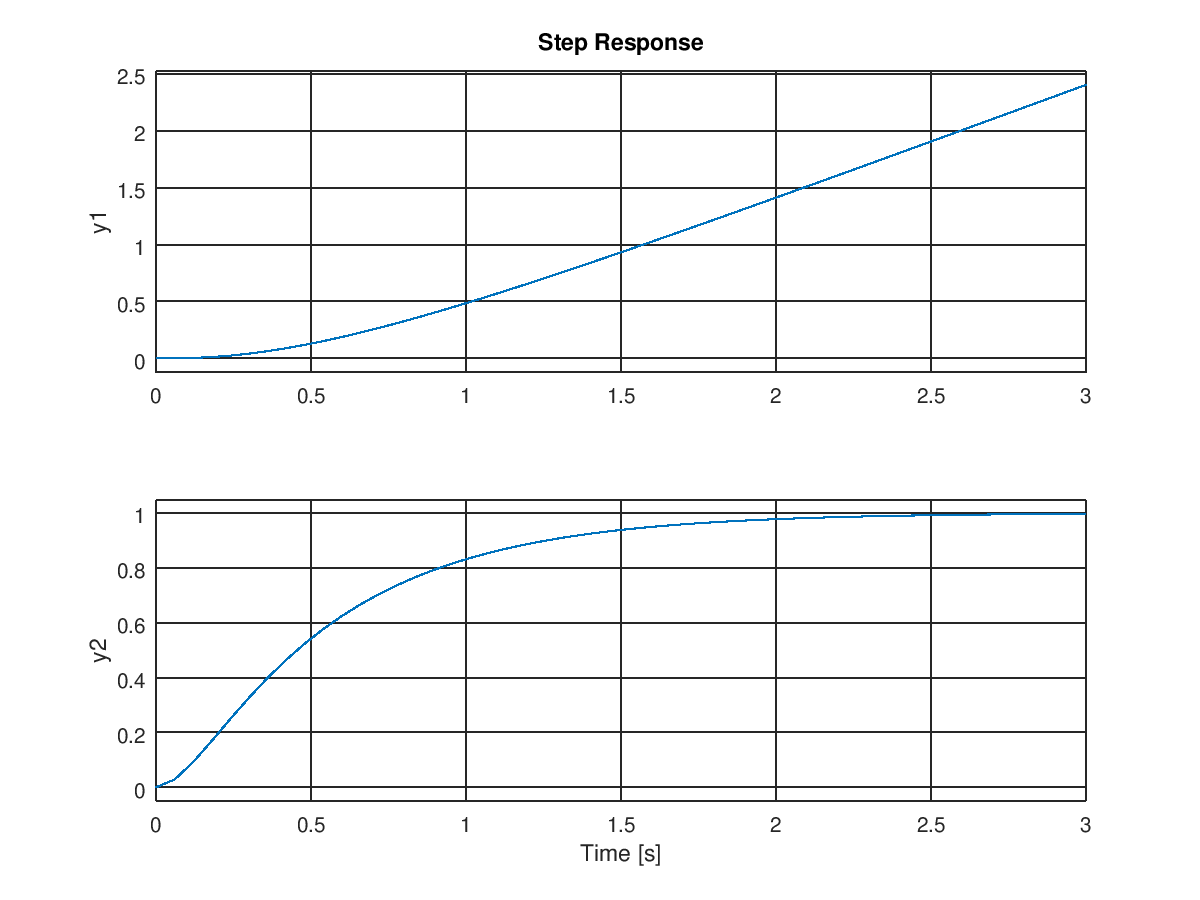
\includegraphics[width=\textwidth]{Images/question_3_output_response_kp_1.png}
	\caption{Output response with the addition of proportional control where $K_p = 1$to a step input}
	\label{fig:question_3_output_response_kp_1}
\end{figure}

\begin{figure}[H]
	\centering
	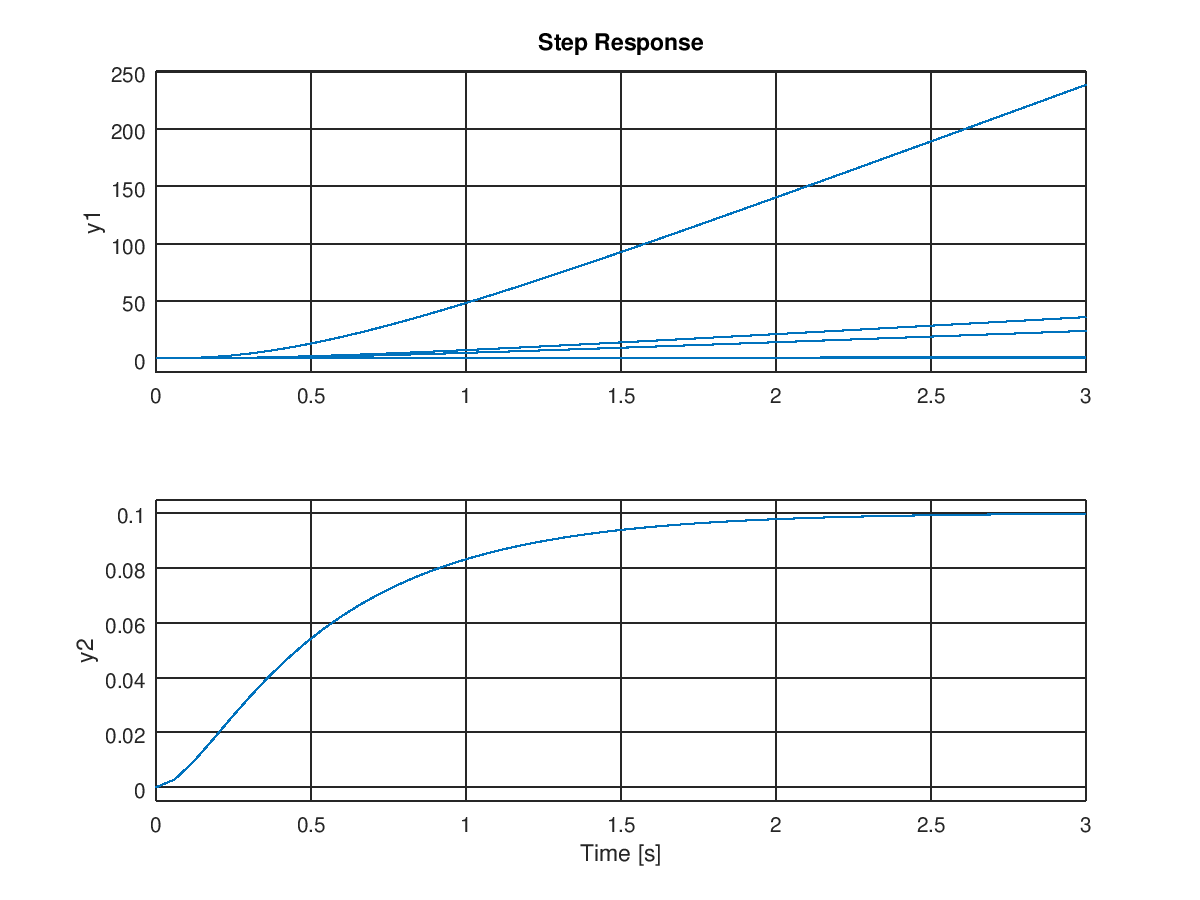
\includegraphics[width=\textwidth]{Images/question_3_output_response_kp_01.png}
	\caption{Output response with the addition of proportional control where $K_p = 0.1$to a step input}
	\label{fig:question_3_output_response_kp_01}
\end{figure}

Figures \ref{fig:question_3_output_response_kp_1} and \ref{fig:question_3_output_response_kp_01} show responses that increase the settling time of the response but gives a steady state error that is unacceptable (the settling value of the speed of the motor seems to take on the value of the proportional constant $K_p$). 

Why is it that the error is so bad ?

\section{Question 4} % (fold)
\label{sec:question_4}
The code that produces the proportional and integral controller applied to the system with transfer function $\frac{Rb+K^2}{(JL)s^3+(Lb+RJ)s+Rb+K}$ is shown below \\ 
\noindent
\texttt{G = tf([R*b+K\^2],[J*L (L\*b+R\*J) R\*b+K]);}\\
\texttt{D = tf([Kp Ki],[1 0])}\\
\texttt{H = feedback(D \* G)}\\
\texttt{step(H)}\\

The step response to a proportional constant and a integral constant of 10 is shown by Figure \ref{fig:question_4_output_response_pi}

\begin{figure}[H]
	\centering
	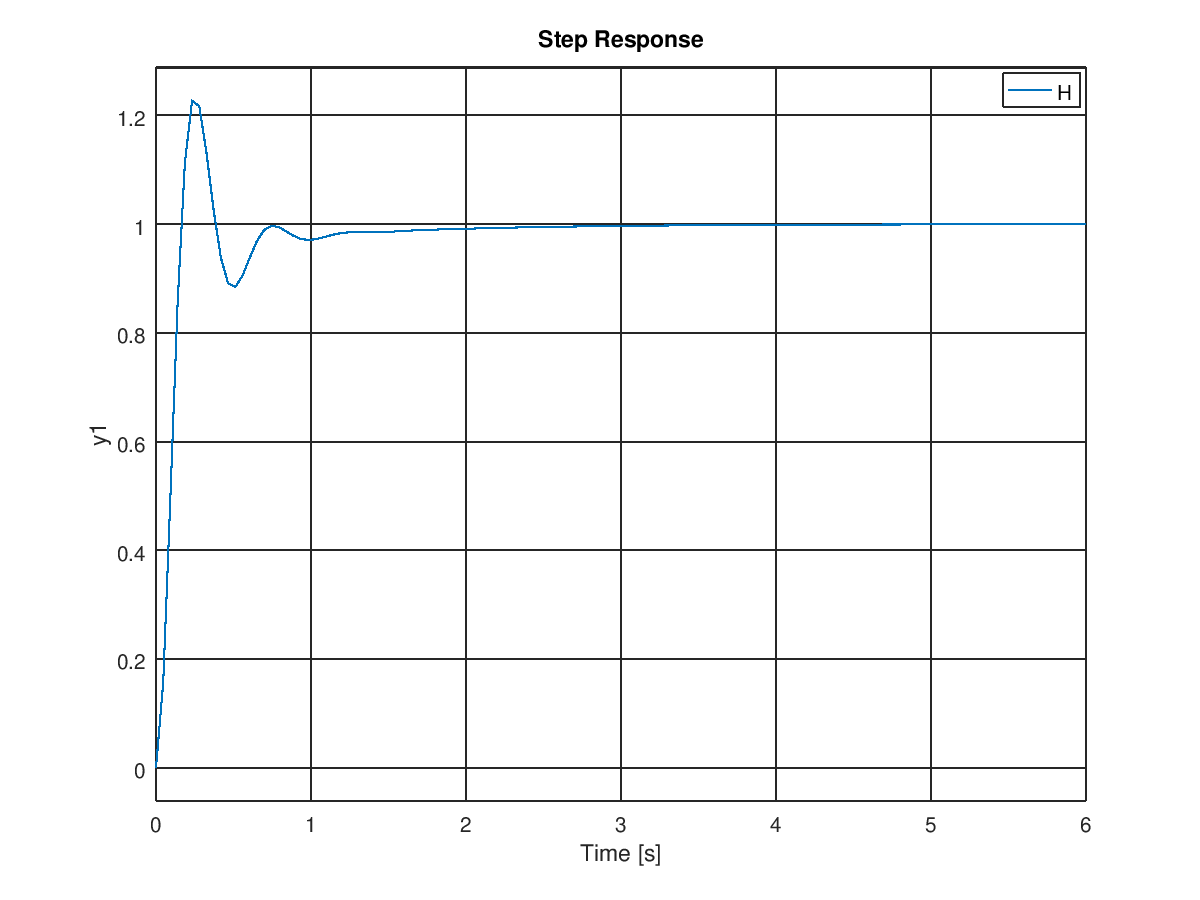
\includegraphics[width=\textwidth]{Images/question_4_output_response_PI.png}
	\caption{Output response of system with $K_p=K_i=10$}
	\label{fig:question_4_output_response_pi}
\end{figure}

For a proportional and derivative controller the code used to produce the proportional and integral controller can be modified as follows below to give the response as shown by Figure (reference)\\
\noindent
\texttt{G = tf([R\*b+K\^2],[J\*L (L\*b+R\*J) R\*b+K]);}
\texttt{D = tf([Kd Kp],[1])}
\texttt{H = feedback(D \* G)}
\texttt{step(H)}

\begin{figure}[H]
	\centering
	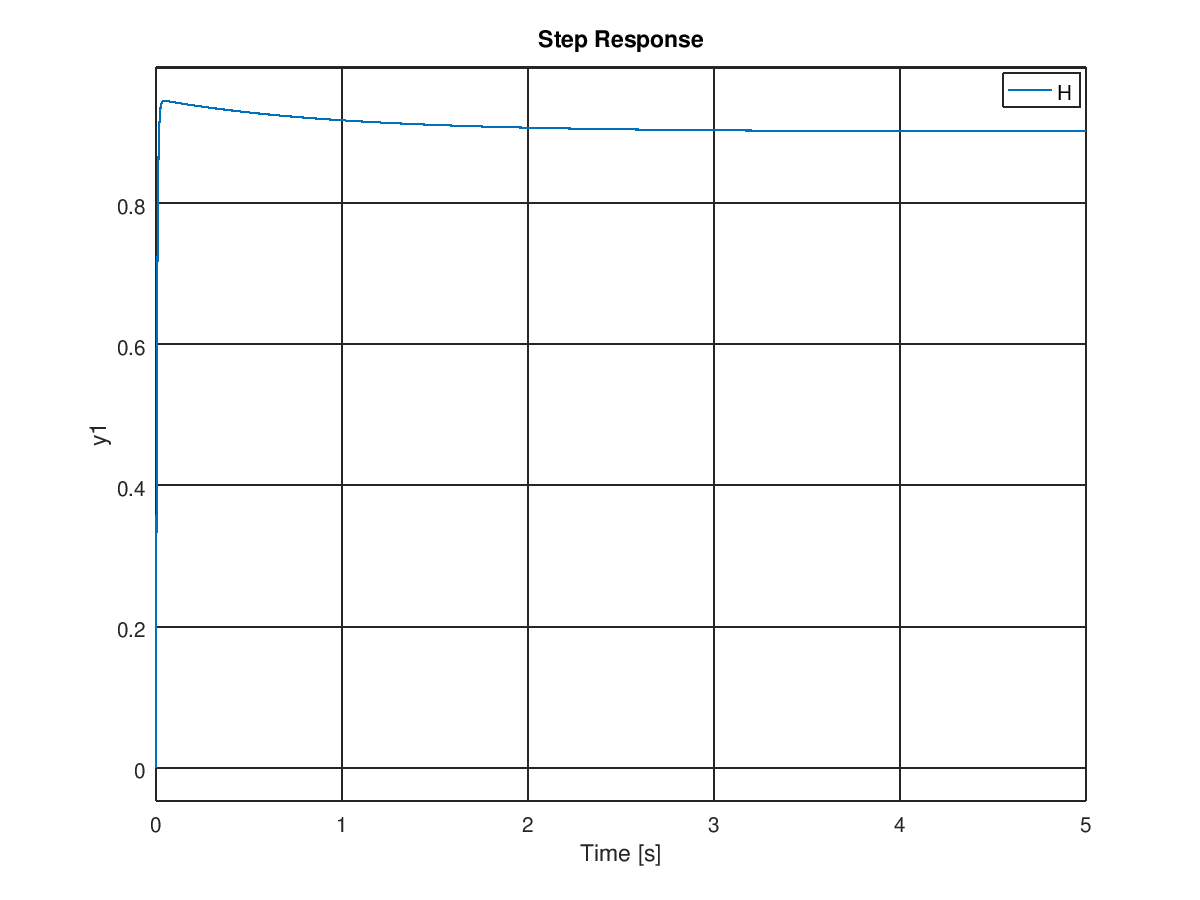
\includegraphics[width=\textwidth]{Images/question_4_output_response_PD.png}
	\caption{Output response of system with $K_p=K_d=10$}
	\label{fig:question_4_output_response_pd}
\end{figure}

Again the code can be modified to include an integral term as well to form the PID controller substituting \texttt{D = tf([Kd Kp Ki],[1 0])} in the code above. The response that is then produced is given by Figure (reference)

\begin{figure}[H]
	\centering
	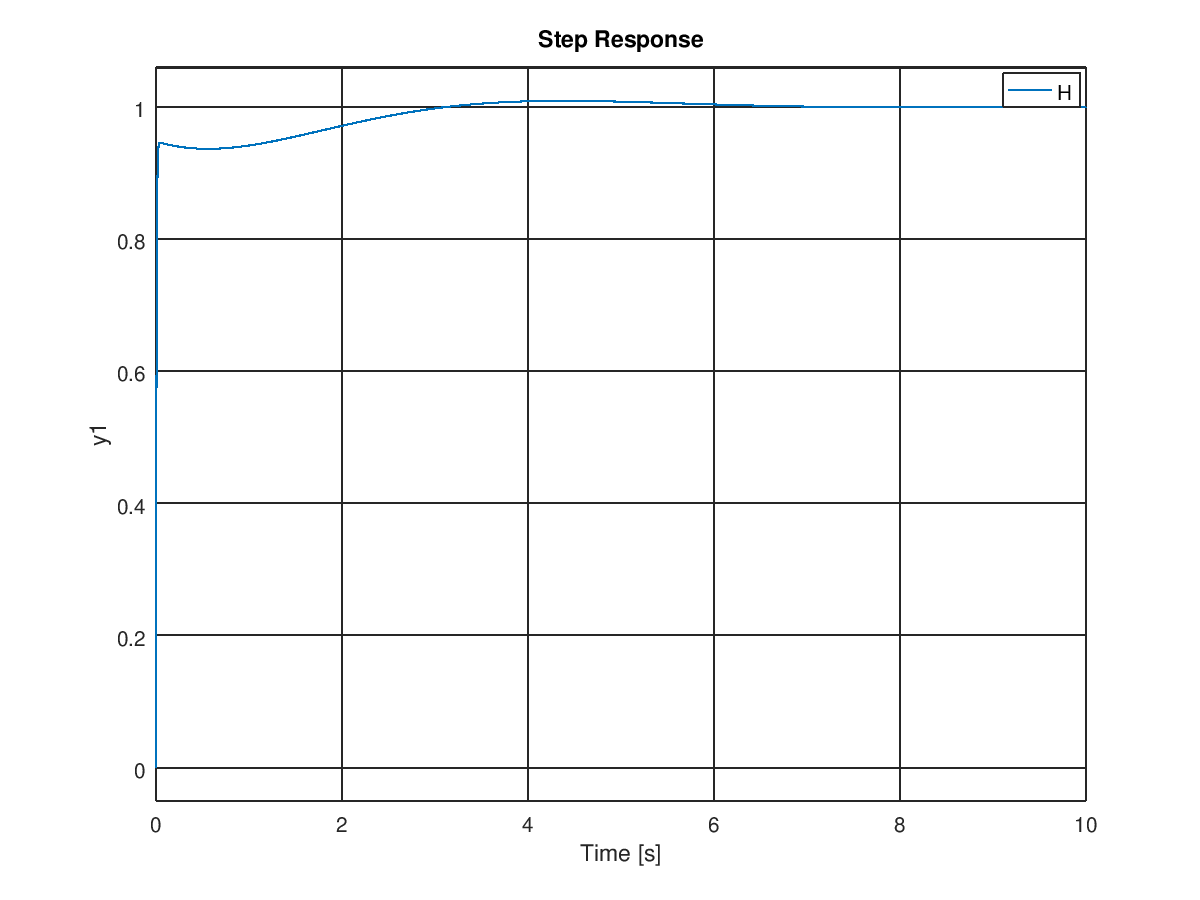
\includegraphics[width=\textwidth]{Images/question_4_output_response_PID.png}
	\caption{Output response of system with $K_p=K_d=K_d=10$}
	\label{fig:question_4_output_response_pid}
\end{figure}

\begin{center}
	\textit{Throughout the use of the different controllers, gains were chosen to be equal and given as 10 for demonstration purposes of the effect of the different controllers}
\end{center}

% section question_4 (end)


\end{document}

